\documentclass[10pt,a4paper,twoside]{article}
\usepackage[english]{babel}
\usepackage{amsmath,amssymb,amsfonts,textcomp}
\usepackage{graphicx}
\usepackage{float,flafter}
\usepackage[hidelinks]{hyperref}
\usepackage[utf8]{inputenc}
% Layout from the supplied hw2_report.tex, with equal recto/verso margins.
\setlength\paperwidth{20.999cm}\setlength\paperheight{29.699cm}\setlength\voffset{-1in}\setlength\hoffset{-1in}\setlength\topmargin{1.499cm}\setlength\headheight{12pt}\setlength\headsep{0cm}\setlength\footskip{1.131cm}\setlength\textheight{25cm}\setlength\oddsidemargin{2.499cm}\setlength\evensidemargin{2.499cm}\setlength\textwidth{15.999cm}
\graphicspath{{figures/}}
\hypersetup{pdftitle={Homework 4: Vital Visions},pdfauthor={Yuntian Wu}}
\begin{document}
\begin{center}
\hrule
\vspace{.4cm}
{\bf {\Huge Homework 4: Vital Visions}}
\vspace{.2cm}
\end{center}
\noindent{\bf Yuntian Wu} (yuntianw@andrew.cmu.edu) \hfill 6 Nov 2026\par
\hrule
\renewcommand{\contentsname}{Table of Contents}
\tableofcontents
\vspace{.4cm}
\noindent\textbf{Experiment scope.} Part 1 uses a real finger-over-camera recording. Part 2 reports actual medical-image fine-tuning. Part 3 reports physical screen-camera recordings covering both alpha differences and all four required distances, followed by two faster transmissions. A subsequent live phone test received \texttt{CMU} with a successful CRC check, documented in the accompanying screen-recorded demo. This demonstration is separate from the offline BER measurements. Code and report sources are available in the public GitHub repository linked in Section~4.

\clearpage
\section{Part 1: Smartphone-Based Heart Rate Monitoring}
\subsection{Capture and signal processing}
I recorded my finger covering the rear camera of an iPhone 17 Pro Max with the flash continuously on. The recording contains 882 frames at $1080\times1920$ resolution and lasts approximately 36.765 s. Decoded timestamps give a sampling rate of $F_s=24$ Hz, rather than the 30 Hz used in the assignment example.

For each frame, I converted the full image to grayscale and computed the spatial mean. After excluding the first two seconds, I resampled the timestamped measurements onto a uniform grid. The analyzed sequence contains $N=834$ samples over 34.75 s. I subtracted the DC mean and applied a third-order Butterworth high-pass filter with a 0.5 Hz cutoff, forward and backward to avoid phase delay. I then applied a Hann window and computed the FFT without zero padding.

\subsection{FFT and heartbeat detection}
I searched for the largest FFT magnitude in $[1,100/60]$ Hz, corresponding to the required 60--100 bpm range. The estimated frequency was $\hat f=1.03597$ Hz, giving $60\hat f=62.16$ bpm. The FFT spacing is $F_s/N=0.02878$ Hz, or approximately 1.73 bpm.

The expected interval between beats, in samples, is
\[
\hat P=\frac{F_s}{\hat f}=\frac{24}{1.03597}=23.17.
\]
I used \texttt{scipy.signal.find\_peaks} with a minimum distance of $\lfloor0.65\hat P\rfloor=15$ samples and prominence 0.1170. This distance threshold allows variation around the estimated period. There were 36 detected peaks. Using the mean consecutive peak interval gave $60/\overline{\Delta t}=62.15$ bpm.

\begin{figure}[H]
\centering
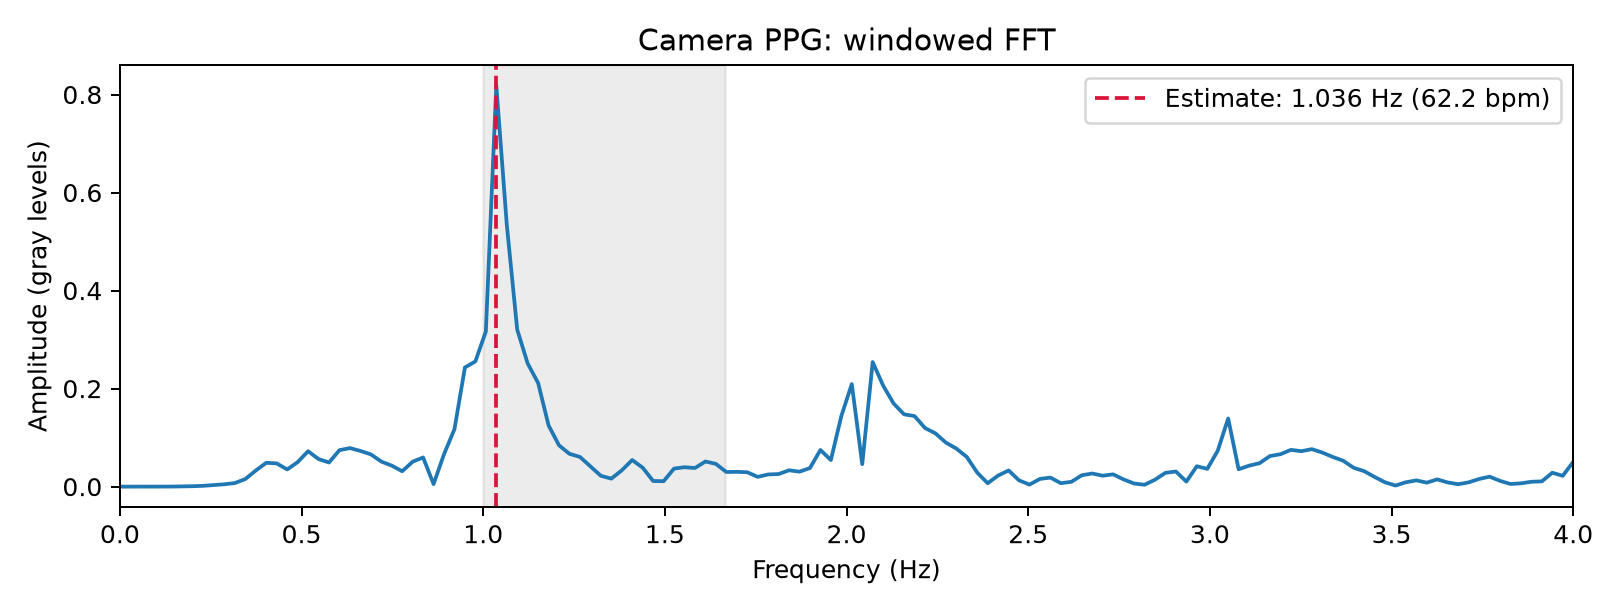
\includegraphics[width=.90\textwidth,height=4.0cm,keepaspectratio]{heart_fft.png}
\caption{FFT of the filtered brightness signal. The selected frequency is 1.036 Hz, corresponding to 62.16 bpm.}
\label{fig:heartfft}
\end{figure}
\begin{figure}[H]
\centering
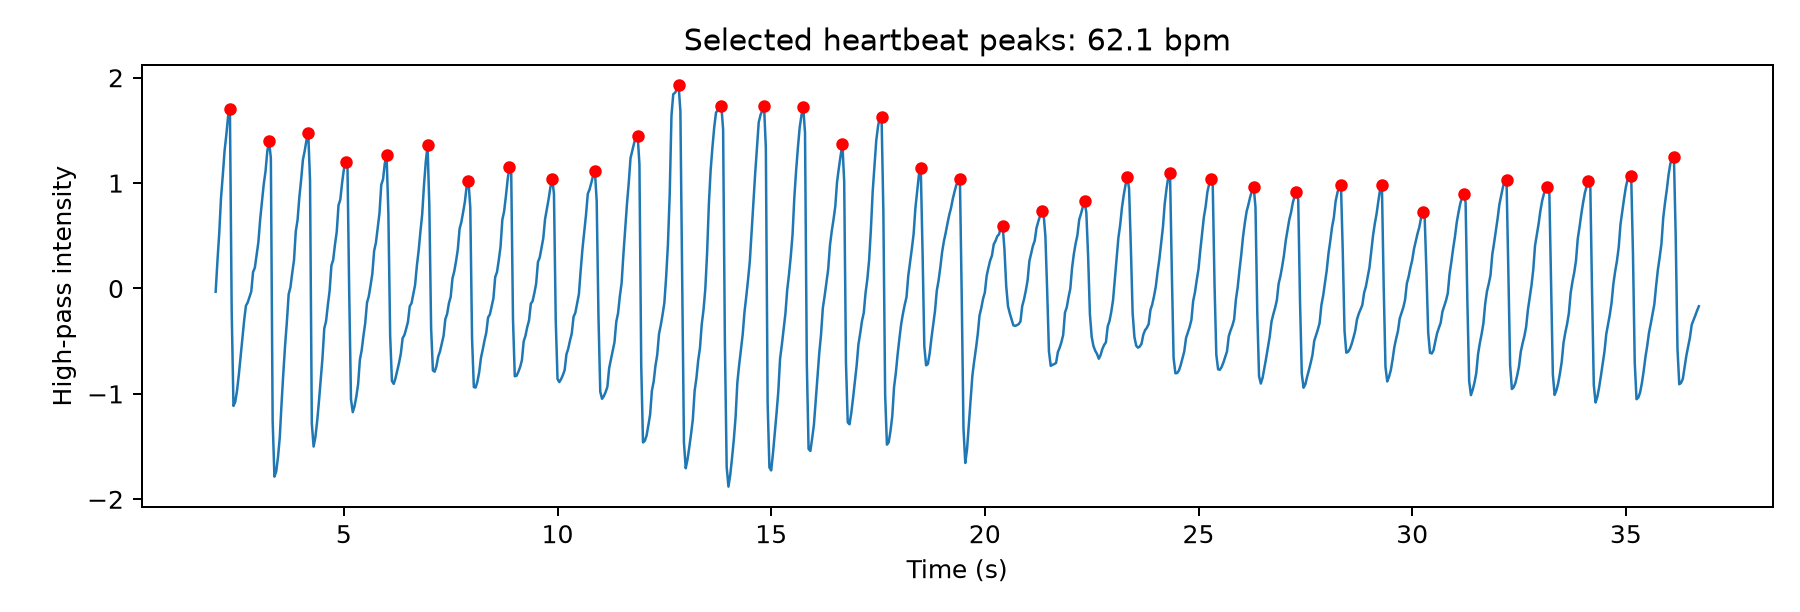
\includegraphics[width=.94\textwidth,height=4.0cm,keepaspectratio]{heart_peaks.png}
\caption{Filtered time-domain signal with detected heartbeat peaks. The peak-interval estimate is 62.15 bpm.}
\label{fig:heartpeaks}
\end{figure}
\subsection{Signal quality and limitations}
The brightness change around 19--20 s coincided with a slight finger movement; this segment and its peaks were retained. Agreement between the two estimates does not establish accuracy without a reference measurement. The search was restricted to 60--100 bpm. No no-flash or controlled-pressure experiment was performed.

\clearpage
\section{Part 2: Fine-Tuning a Vision Model for Medical Images}
\subsection{Model and dataset}
I selected an ImageNet-pretrained ResNet-18 with \texttt{IMAGENET1K\_V1} weights and replaced its classifier with a seven-output linear layer. The dataset was DermaMNIST from MedMNIST, based on HAM10000 dermatoscopic images. I retained the official split: 7,007 training, 1,003 validation and 2,005 test images. Native $28\times28$ RGB images were resized to $224\times224$ and normalized with the ImageNet mean and standard deviation. Random horizontal and vertical flips were applied only during training.
\subsection{Training setup}
Training ran on a local NVIDIA GeForce RTX 4070 with PyTorch 2.8.0+cu129, seed 42 and batch size 64. AdamW used weight decay $10^{-4}$. Cross-entropy class weights were computed as $w_c=N_{\mathrm{train}}/(7n_c)$ using training labels only.
\begin{table}[H]
\centering
\begin{tabular}{lll}
\hline
Epochs & Trainable components & Learning rate \\
\hline
1 & New classifier & $10^{-3}$ \\
2--6 & Last residual block (\texttt{layer4}) & $10^{-4}$ \\
2--6 & Classifier & $3\times10^{-4}$ \\
\hline
\end{tabular}
\caption{Two-stage fine-tuning. Earlier layers and BatchNorm running statistics remained fixed.}
\end{table}
The checkpoint with the highest validation accuracy was selected at epoch 6, before test evaluation. The accompanying self-contained Colab-compatible notebook contains actual local execution outputs; these outputs were not produced by a Google Colab cloud session.
\subsection{Validation and test results}
\begin{table}[H]
\centering
\begin{tabular}{lrr}
\hline
Metric & Validation ($n=1{,}003$) & Test ($n=2{,}005$) \\
\hline
Accuracy & $66.60\%$ & $67.73\%$ \\
Balanced accuracy & $53.81\%$ & $56.23\%$ \\
Macro one-vs-rest AUC & 0.9127 & 0.9144 \\
Macro F1 & 0.4652 & 0.4550 \\
\hline
\end{tabular}
\caption{Metrics from the selected checkpoint. Balanced accuracy is the mean recall across the seven classes.}
\label{tab:medical}
\end{table}
\begin{figure}[H]
\centering
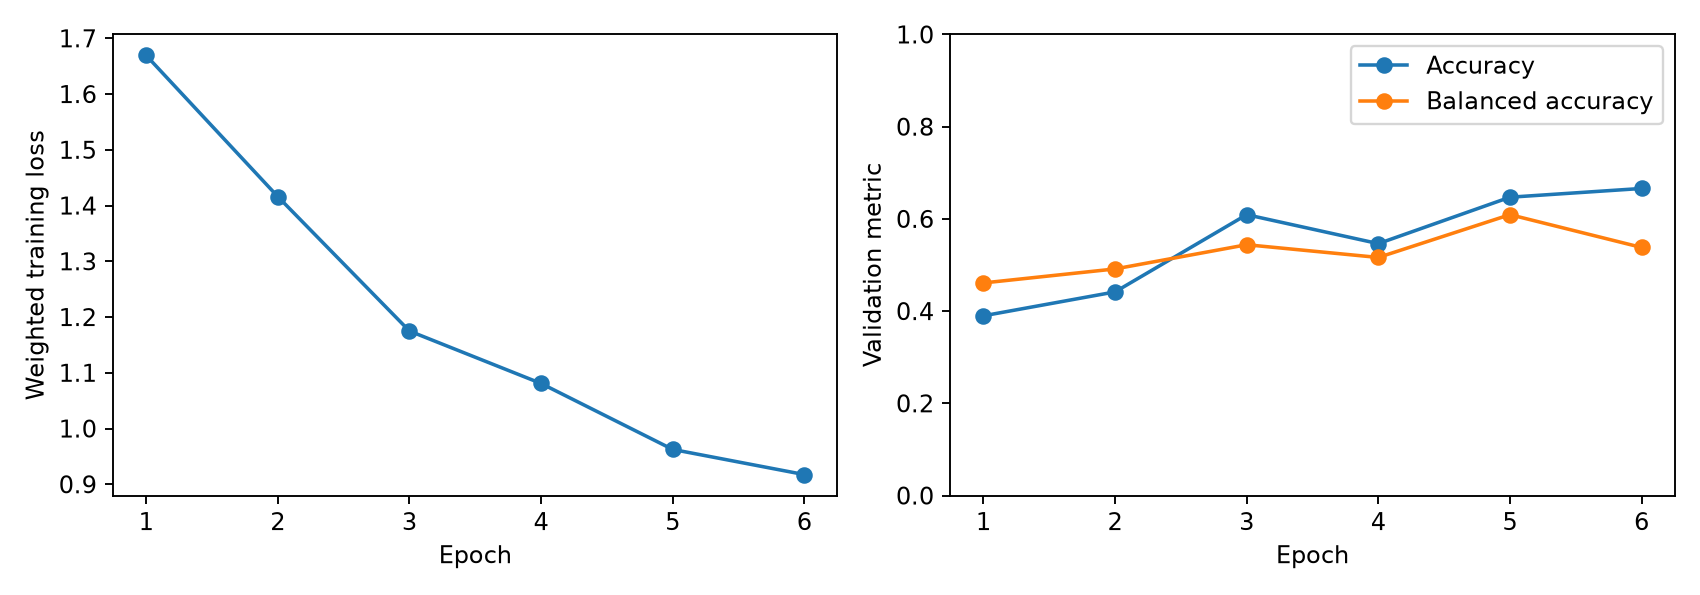
\includegraphics[width=\textwidth,height=7.1cm,keepaspectratio]{learning_curves.png}
\caption{Weighted training loss and validation accuracy/balanced accuracy over six epochs. Checkpoint selection used validation accuracy.}
\label{fig:learning}
\end{figure}

\clearpage
\subsection{Class errors and interpretation}
\begin{figure}[H]
\centering
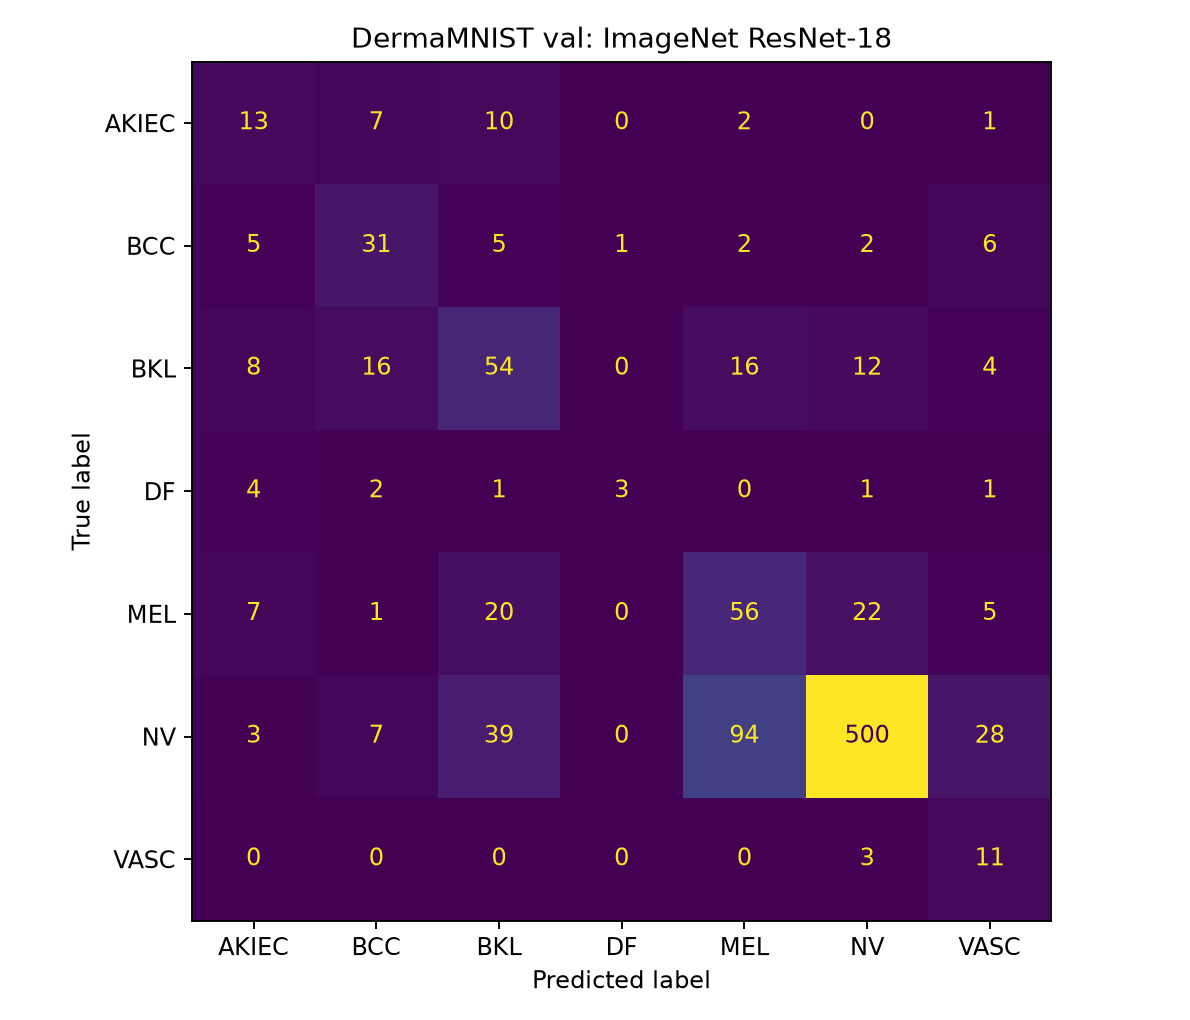
\includegraphics[width=.83\textwidth,height=11.7cm,keepaspectratio]{val_confusion.png}
\caption{Validation confusion matrix. AKIEC: actinic keratoses and intraepithelial carcinoma; BCC: basal cell carcinoma; BKL: benign keratosis-like lesions; DF: dermatofibroma; MEL: melanoma; NV: melanocytic nevi; VASC: vascular lesions.}
\label{fig:confusion}
\end{figure}
Melanocytic nevi account for 671 of the 1,003 validation examples. Always predicting this class would achieve $66.90\%$ accuracy, but only $1/7=14.29\%$ balanced accuracy. The fine-tuned model's overall accuracy is slightly below this majority-class baseline, while its balanced accuracy is higher. These results show broader class coverage rather than improved total accuracy over that baseline.

The confusion matrix shows substantial confusion among melanoma, benign keratosis-like lesions and melanocytic nevi. Inverse-frequency weighting changes the tradeoff between frequent and rare classes. Validation balanced accuracy was higher at epoch 5 than epoch 6, although epoch 6 was selected by accuracy. Thus, the checkpoint selection metric affects the final tradeoff.

Resizing native $28\times28$ images cannot restore fine clinical detail. The experiment uses one seed and one official split, without an external evaluation dataset. Patient identity overlap was not independently audited from the source patient IDs. This is an educational transfer-learning experiment, not a clinically validated diagnostic system.

\clearpage
\subsection{Optional ROC and feature visualization}
\begin{figure}[H]
\centering
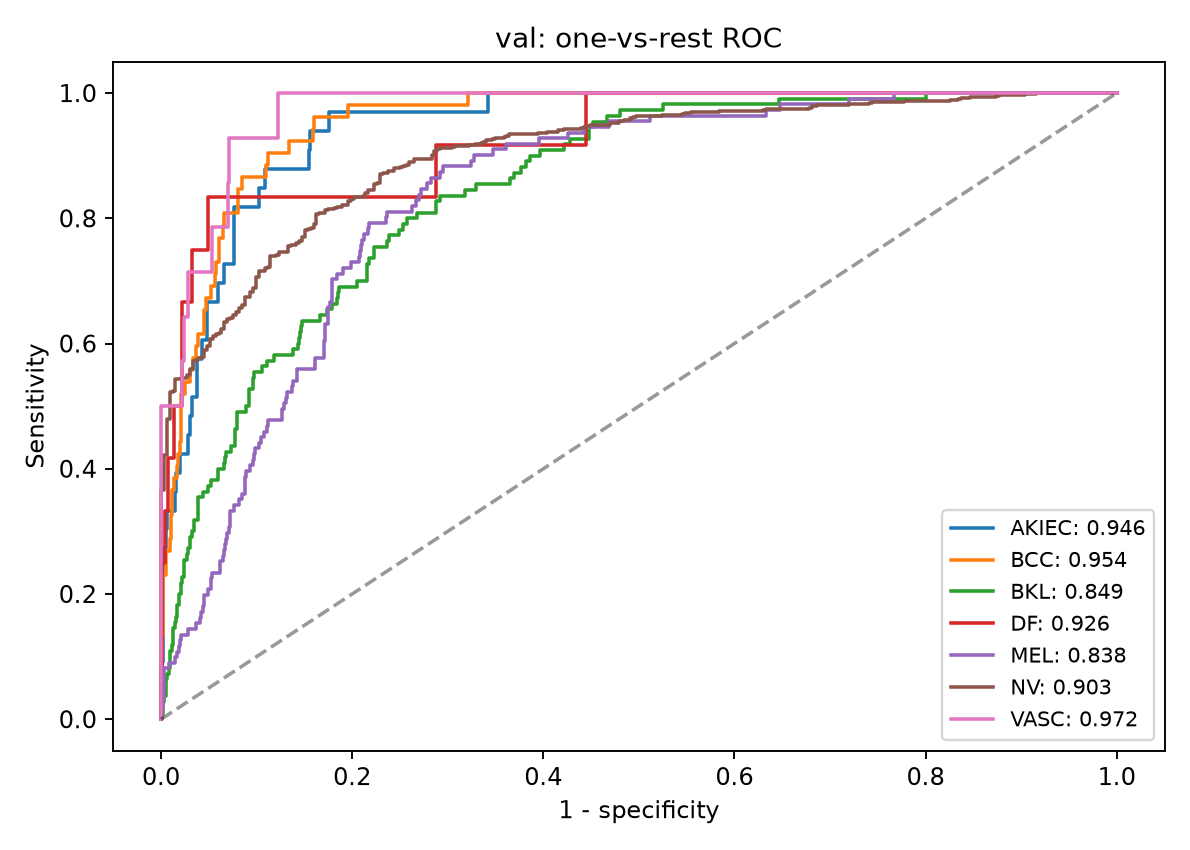
\includegraphics[width=.83\textwidth,height=9.4cm,keepaspectratio]{val_roc.png}
\caption{One-vs-rest validation ROC curves. The axes are $1-\mathrm{specificity}$ and sensitivity; the legend reports class AUCs. Macro AUC is 0.9127.}
\label{fig:roc}
\end{figure}
\begin{figure}[H]
\centering
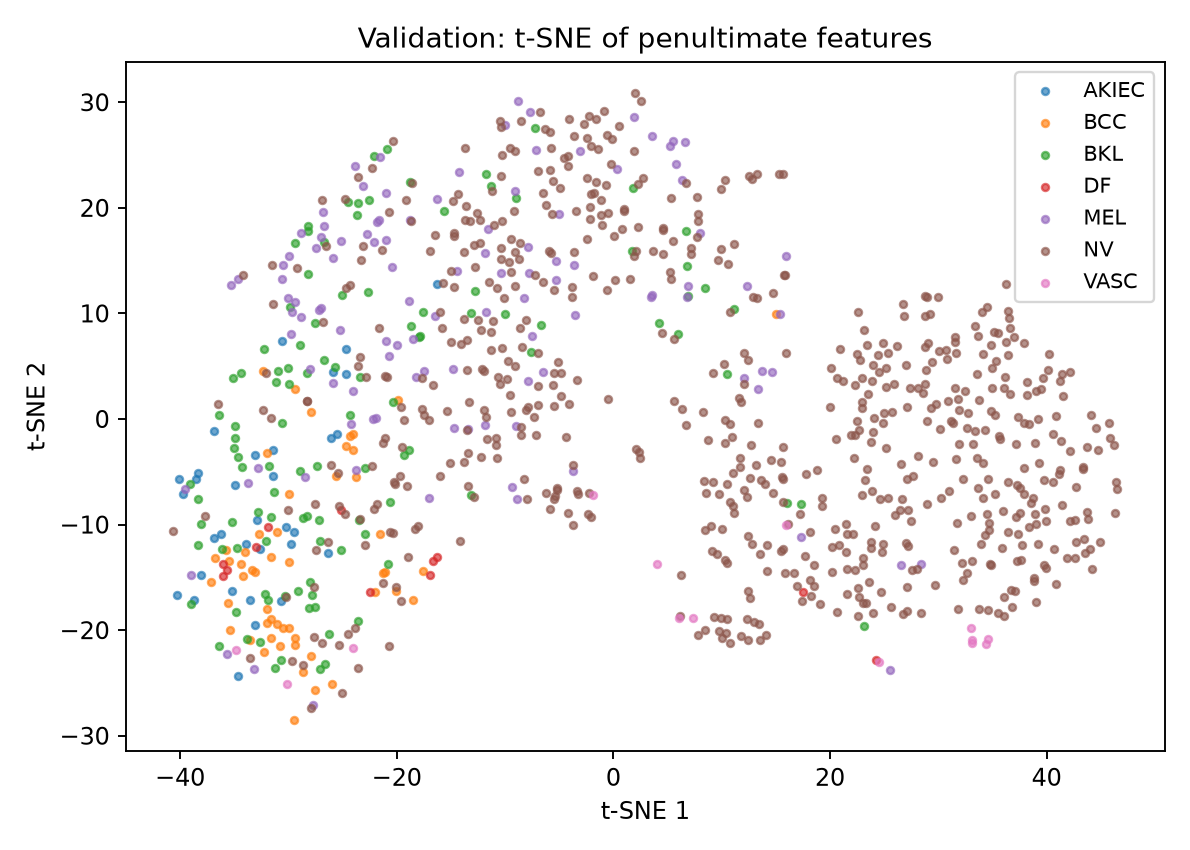
\includegraphics[width=.83\textwidth,height=9.4cm,keepaspectratio]{val_tsne.png}
\caption{t-SNE of the 512-dimensional penultimate-layer validation features, with perplexity 30 and seed 42. Colors indicate ground-truth classes.}
\label{fig:tsne}
\end{figure}
ROC curves evaluate score ranking over varying thresholds, whereas classification accuracy uses the argmax class. t-SNE is descriptive; visual separation alone does not measure classification performance.

\clearpage
\section[Part 3: Screen-Camera Communication Using Alpha]{Part 3: Screen-Camera Communication\\Using the Alpha Channel}
\subsection{Transmitter and receiver}
I displayed a static mountain illustration over black and varied its opacity as
\[
\alpha(t)=1-\frac{\Delta\alpha}{2}+\frac{\Delta\alpha}{2}\sin(2\pi f_b t),
\qquad \alpha(t)\in[1-\Delta\alpha,1].
\]
For binary frequency-shift keying (BFSK), bit 0 uses $f_0=2/T$ and bit 1 uses $f_1=4/T$, where $T$ is the bit duration. The baseline used $T=1$ s, so the two frequencies were 2 and 4 Hz. The screen animation ran at approximately 60 Hz and the phone videos at approximately 30 frames/s.

Each transmission sent the UTF-8 message \texttt{CMU}. A packet comprised a 13-bit public Barker preamble, an 8-bit payload-length field, 24 payload bits and an 8-bit CRC (polynomial \texttt{0x07}): 53 bits. The offline receiver averaged an image-interior region. Within each symbol, regression included an offset, linear drift and sine/cosine terms for each candidate tone; the decoder selected the better tone fit. Synchronization used only the public preamble, not agreement with the message payload.
\subsection{Physical baseline results}
I recorded one packet for each combination of $d\in\{20,40,80,120\}$ cm and $\Delta\alpha\in\{0.1,0.5\}$. The assignment's BER and correct-bit rate were calculated as
\[
\mathrm{BER}=1-\frac{N_{\mathrm{correct}}}{N_{\mathrm{sent}}},
\qquad R_{\mathrm{correct}}=\frac{N_{\mathrm{correct}}}{t_{\mathrm{packet}}}.
\]
These quantities include preamble, length and CRC bits; payload-only throughput is reported separately.
\begin{table}[H]
\centering
\begin{tabular}{rcccc}
\hline
Distance & BER & BER & Correct-bit rate & Message \\
(cm) & $\Delta\alpha=0.1$ & $\Delta\alpha=0.5$ & (bit/s, both) & (both) \\
\hline
20 & $0^{*}$ & 0 & 1.00 & \texttt{CMU} \\
40 & 0 & 0 & 1.00 & \texttt{CMU} \\
80 & 0 & 0 & 1.00 & \texttt{CMU} \\
120 & 0 & 0 & 1.00 & \texttt{CMU} \\
\hline
\end{tabular}
\caption{Eight physical baseline transmissions at 1 raw bit/s. Each entry represents one 53-bit packet.}
\label{tab:communication}
\end{table}
\noindent\textit{$^{*}$The original transmitter log for 20 cm/$\Delta\alpha=0.1$ was not saved. Its bits were independently decoded and passed CRC. BER uses the fixed \texttt{CMU} protocol configuration specified before recording and is conditional on that configuration. No transmitter log was reconstructed. The other seven trials have original logs.}

All eight baseline packets decoded as \texttt{CMU} and passed CRC: 0 incorrect bits among 424 frame bits. Correct-bit rate was 1.00 bit/s. Useful payload throughput was $24/53=0.453$ bit/s, excluding setup time and pauses.
\subsection{Recording order and visual observation}
The 80 cm video contains $\Delta\alpha=0.5$ followed by 0.1; the 120 cm baseline video contains 0.1 followed by 0.5. This order matches the transmitter timestamps. Each video was analyzed in two time windows without re-encoding; each full 53 s packet fit within its window. Both alpha settings produced noticeable flicker to the naked eye at the baseline rate. No separate visibility score was recorded at each distance.

\clearpage
\subsection{BER, data rate and signal evidence}
\begin{figure}[H]
\centering
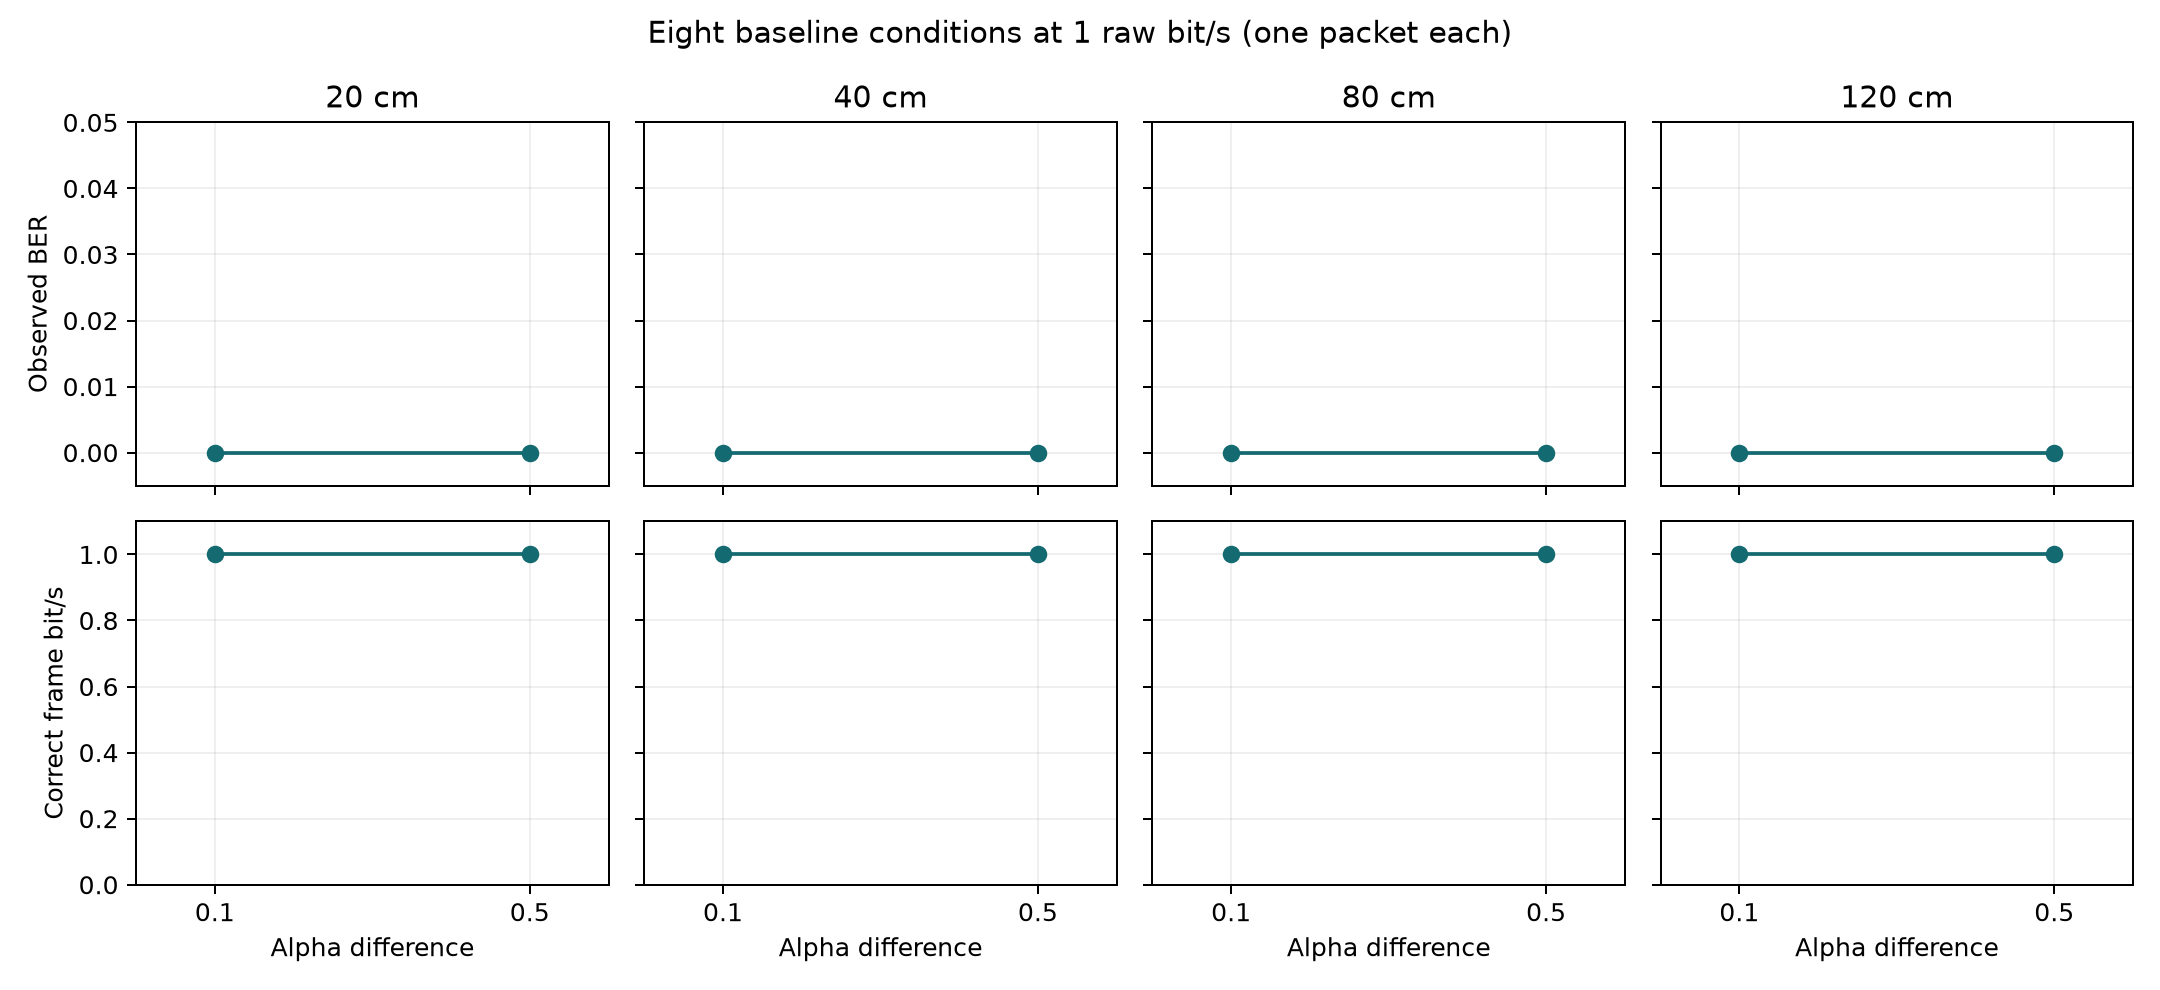
\includegraphics[width=\textwidth,height=8.1cm,keepaspectratio]{baseline_matrix.png}
\caption{Observed BER and correct-bit rate versus alpha difference at the four distances. Each point is one packet at 1 raw bit/s. The qualified reference for 20 cm/0.1 is described with Table~\ref{tab:communication}.}
\label{fig:baseline}
\end{figure}
\begin{figure}[H]
\centering
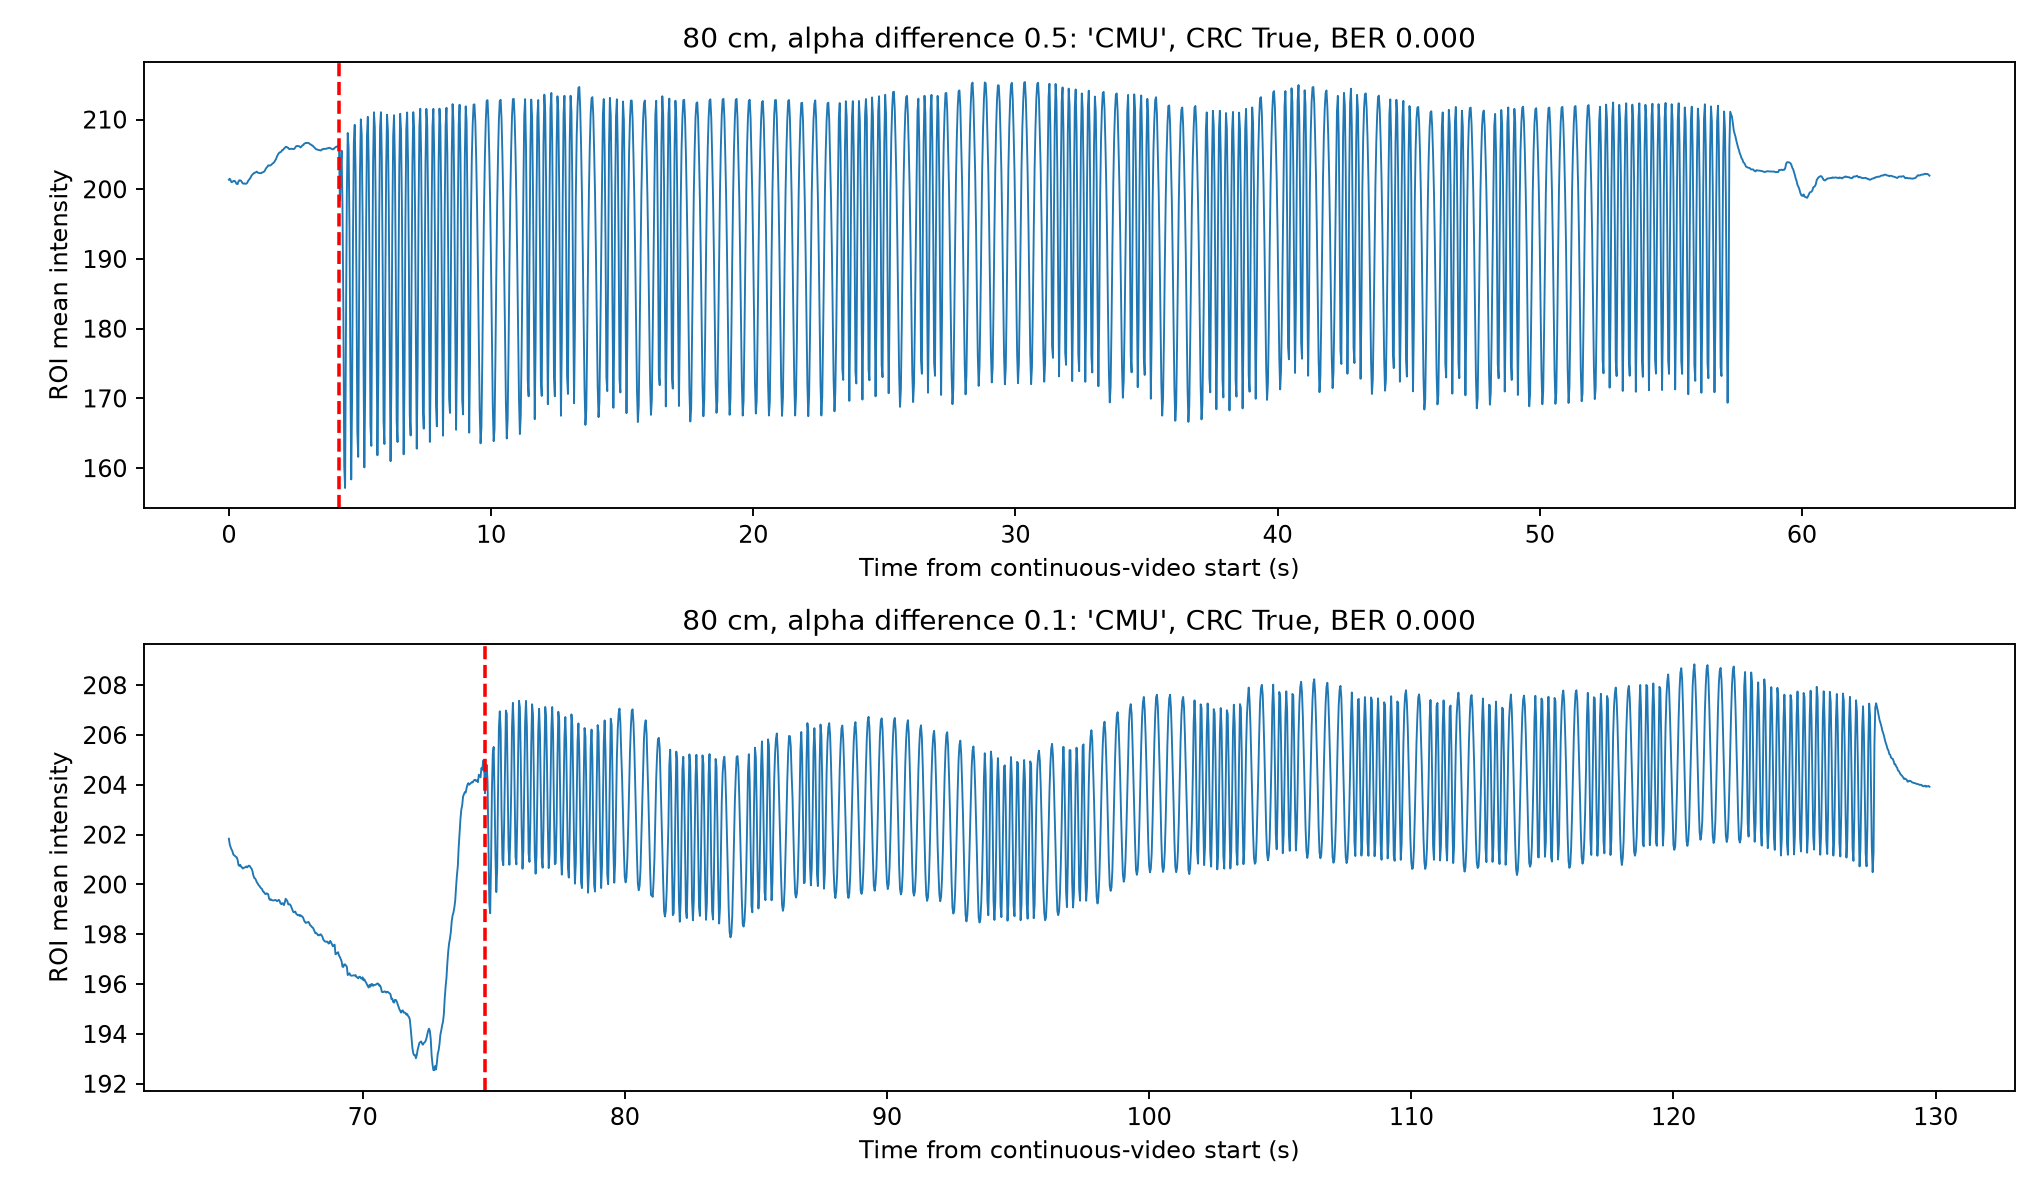
\includegraphics[width=\textwidth,height=7.7cm,keepaspectratio]{d80_transmissions.png}
\caption{Brightness traces from the continuous 80 cm recording: $\Delta\alpha=0.5$ followed by 0.1. Dashed lines indicate preamble-based packet starts. Gradual brightness changes were retained.}
\label{fig:signal}
\end{figure}
No BER or correct-bit-rate difference was observed across the eight baseline packets. One packet per condition does not establish zero long-run error probability or maximum range. Larger distances used a windowed transmitter with controls visible. Display geometry and ROI size differed across recordings, so distance alone was not isolated. ROIs were chosen from image content before decoding and held fixed across both transmissions within each continuous recording.

\clearpage
\subsection{Higher-rate trials}
The final continuous recording contains two transmissions at 120 cm and $\Delta\alpha=0.1$: first 2 bit/s, then 3 bit/s. The tone pairs were 4/8 Hz and 6/12 Hz, respectively. A fixed image-interior ROI was selected before decoding and used for both segments. Packet starts were estimated at 5.250 s and 43.775 s. The 38.525 s separation agrees with the original transmitter-log separation of 38.551 s to within one 30 fps camera frame. Both complete packets lie inside their assigned analysis windows.
\begin{table}[H]
\centering
\begin{tabular}{rrrrcc}
\hline
Raw rate & Duration & Correct-bit rate & Payload rate & BER & CRC \\
(bit/s) & (s) & (bit/s) & (bit/s) & & \\
\hline
2 & 26.500 & 2.00 & 0.906 & 0 & Pass \\
3 & 17.667 & 3.00 & 1.358 & 0 & Pass \\
\hline
\end{tabular}
\caption{Higher-rate results at 120 cm/$\Delta\alpha=0.1$. Each packet decoded as \texttt{CMU}, with 53 of 53 bits correct.}
\label{tab:fast}
\end{table}
\begin{figure}[H]
\centering
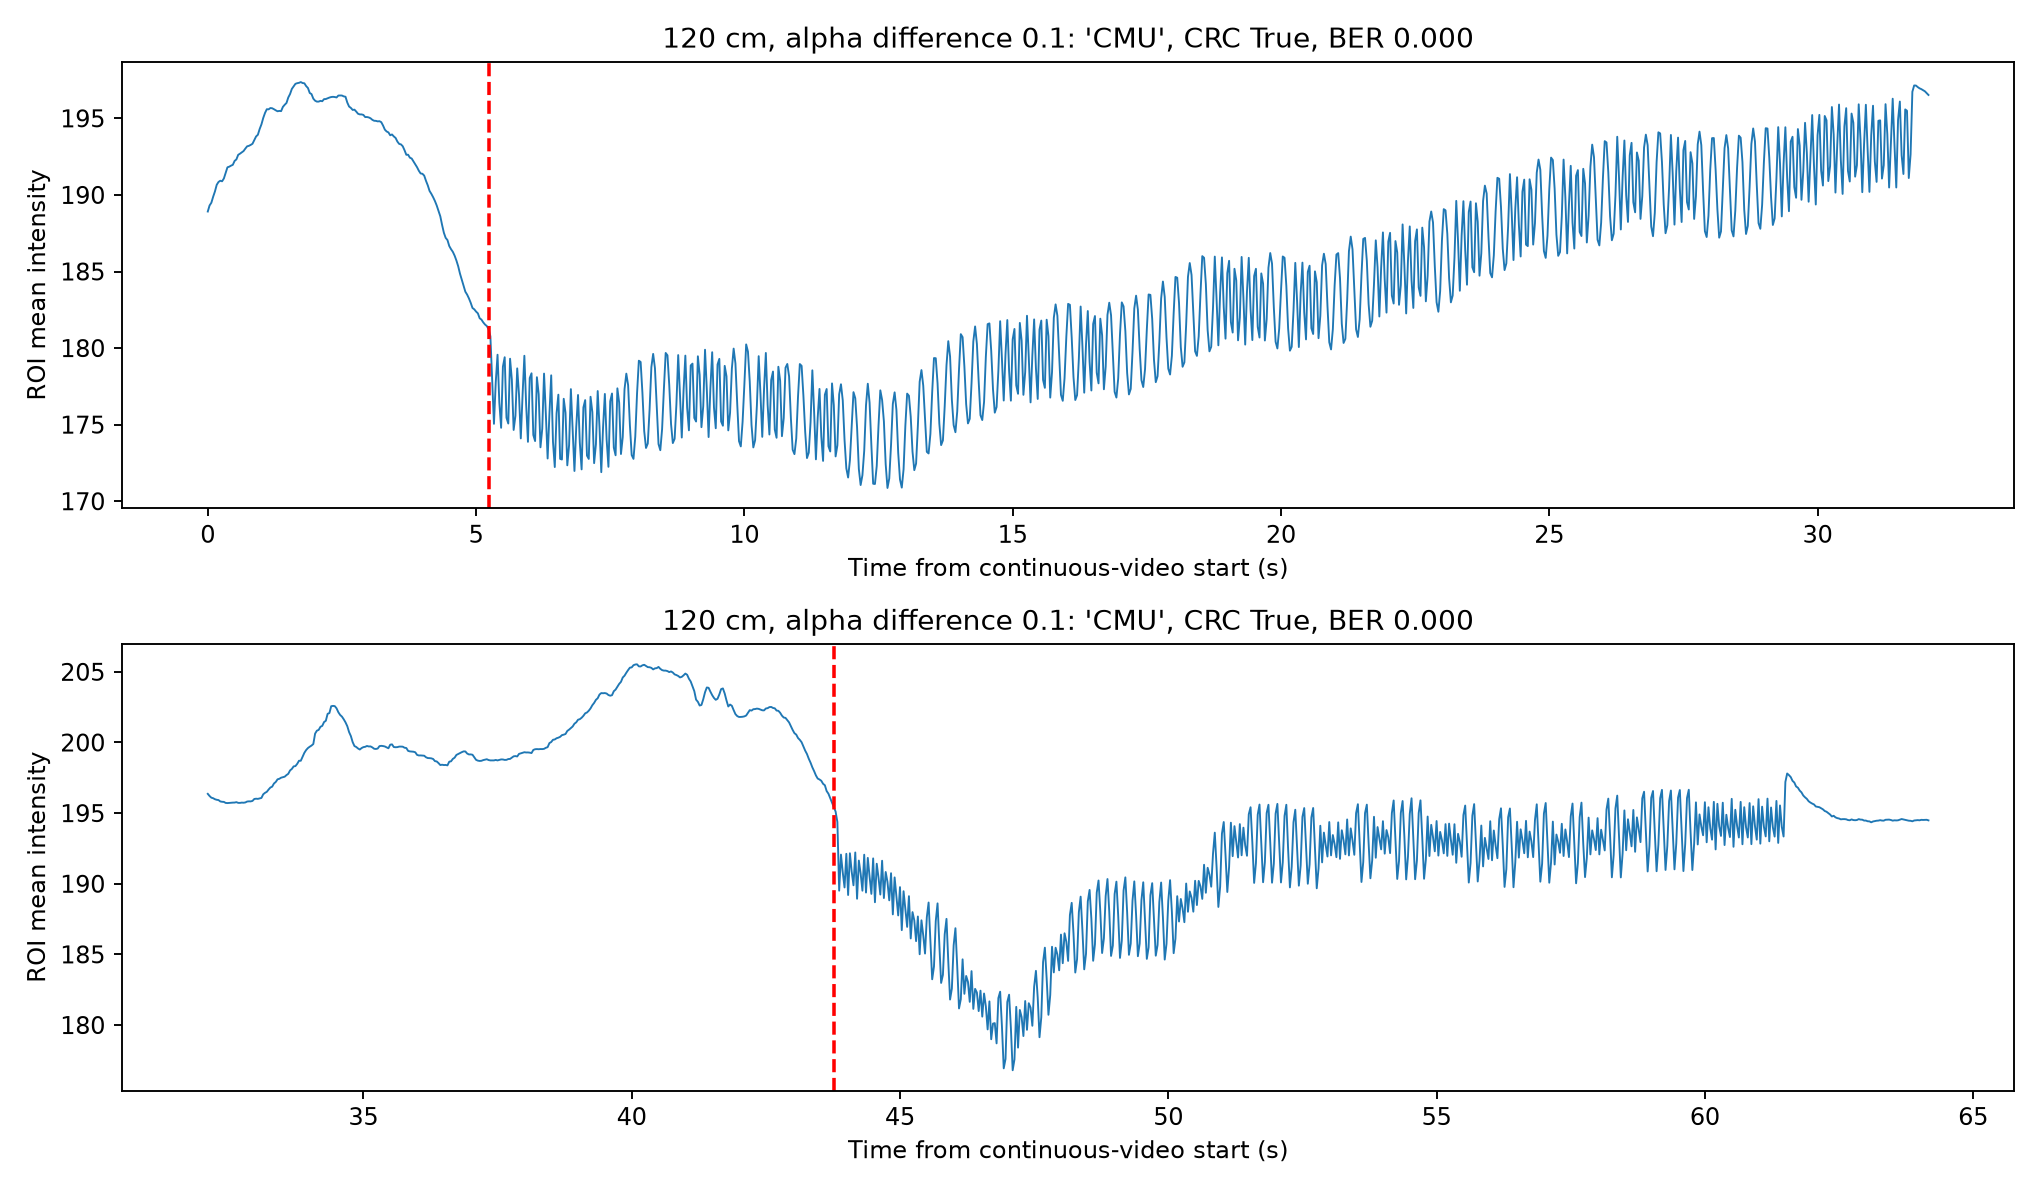
\includegraphics[width=\textwidth,height=6.7cm,keepaspectratio]{fast_transmissions.png}
\caption{The two higher-rate transmissions in the original continuous video. Dashed lines indicate packet starts selected using the public preamble.}
\label{fig:fast}
\end{figure}
The maximum successfully tested raw rate was 3 bit/s in this condition; this does not establish channel capacity or performance at untested combinations. At 30 camera frames/s, the 12 Hz tone has only about 2.5 samples per cycle, making exposure and frame timing relevant. The eight baseline packets and two faster packets contain 530 compared frame bits with no observed errors, subject to the qualified reference for the first baseline recording.

Both alpha differences were visibly flickering at the baseline rate. I also observed noticeable flicker in both the 2 and 3 bit/s recordings. Thus, imperceptible communication was not demonstrated within the tested rates, and a perceptual transition speed was not established.

An additional live phone demonstration is documented in the following subsection. It is reported separately from the 530-bit offline BER comparison above.


\clearpage
\subsection{Recorded real-time phone demonstration}
The accompanying video, \texttt{HW4\_Live\_Demo.mp4}, records live reception on the phone in the English browser interface. The original recording is 77.33 s long at 30 frames/s, with a resolution of $592\times1280$. It is retained without editing or re-encoding.

At approximately 5 s, the visible transmitter controls show a configured distance of 20 cm, $\Delta\alpha=0.1$ and a bit duration of 1 s. The receiver uses the matching bit duration. The configured distance was not independently remeasured from the screen recording. This recorded configuration supersedes the earlier guided 0.5 setting for the demo described here.

\begin{figure}[H]
\centering
\begin{minipage}{.48\textwidth}
\centering
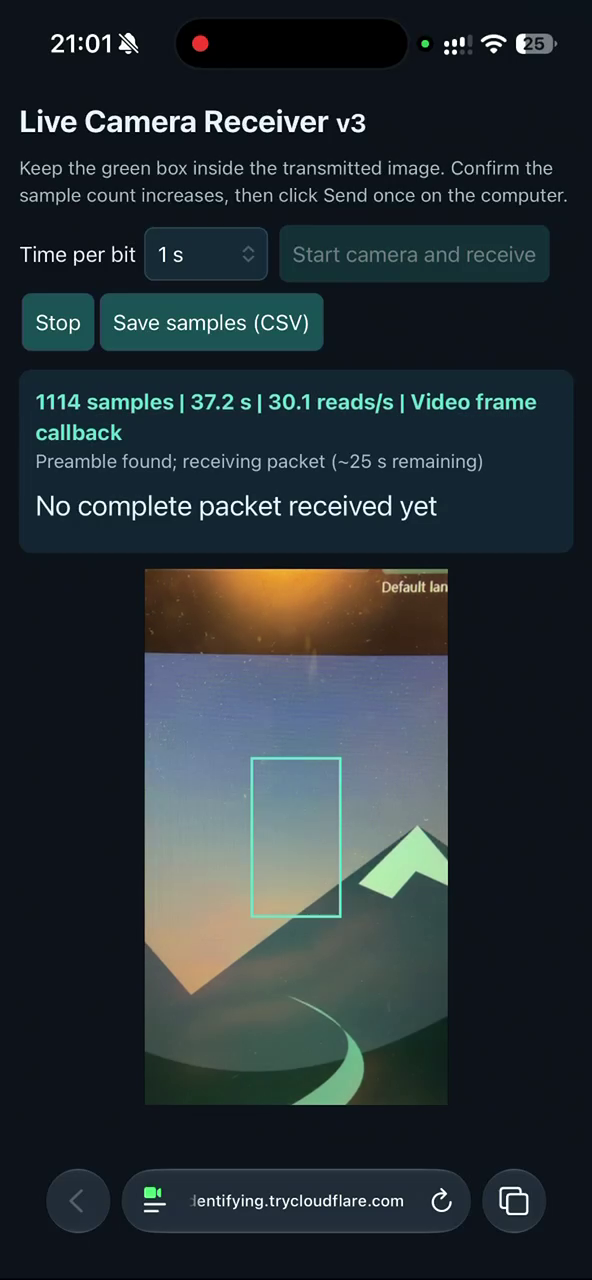
\includegraphics[height=13.1cm,keepaspectratio]{live_progress.png}
\end{minipage}
\hfill
\begin{minipage}{.48\textwidth}
\centering
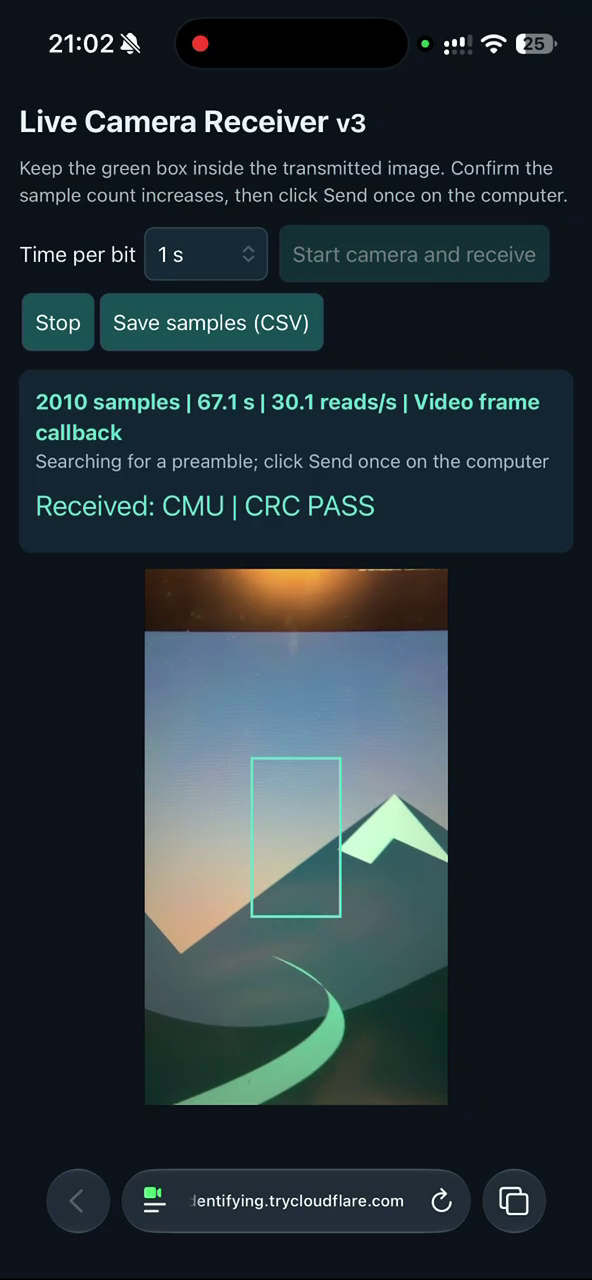
\includegraphics[height=13.1cm,keepaspectratio]{live_success.png}
\end{minipage}
\caption{Unmodified frames extracted at 40 s (left) and 70 s (right) from the supplied screen recording. Left: the receiver has found the preamble and is waiting for the rest of the packet. Right: the interface displays \texttt{Received: CMU | CRC PASS}.}
\label{fig:livedemo}
\end{figure}

The recording shows the sample count increasing and a transition from preamble detection to successful message reception. At the 70 s evidence frame, the receiver reports 2,010 samples over 67.1 s, approximately 30.1 reads/s, and video-frame-callback capture mode. These are displayed receiver diagnostics, not measurements recovered from an exported intensity trace.

The video directly documents a functional live reception, beyond the earlier participant confirmation. No raw live intensity CSV or original transmitter log for this new demo is archived. Therefore, this demo is not used to add bits to the offline BER estimates, estimate channel capacity, or infer performance at untested settings. The demonstration sends one message, \texttt{CMU}; it does not demonstrate multiple different words.


\clearpage
\section{Code and Reproducibility}
\begin{itemize}
\item \texttt{heart\_rate.py}: timestamp-aware grayscale extraction, filtering, FFT and peak detection; outputs in \texttt{results/heart\_rate/IMG\_2324/}.
\item \texttt{finetune.py} and \texttt{HW4\_Part2\_Colab.ipynb}: model training and evaluation; metrics and figures in \texttt{results/finetune/}.
\item \texttt{web/transmitter.html} and \texttt{web/receiver.html}: English-language browser transmitter and receiver. The receiver shows live sampling status, includes a compatibility capture fallback, and decodes in a worker thread. The accompanying demo records a successful live \texttt{CMU}/CRC reception.
\item \texttt{communication.py} and \texttt{decode\_sequence.py}: offline decoding for single and continuous recordings.
\item \texttt{decode\_unlogged.py}: decoding without an original transmitter log.
\item \texttt{summarize\_communication.py}: aggregation of physical trial results.
\end{itemize}
The notebook and result files preserve the numerical record. Real recordings and actual training are distinguished from software/synthetic verification. Raw videos are retained locally and excluded from the source package.

\noindent\textbf{GitHub repository:} \url{https://github.com/GitaTReNt/17-720-HW4-Vital-Visions}.

The public repository contains the code, executed notebook, measured results and report source. Raw phone videos, dataset archives, model weights and temporary runtime files are excluded. The original demo video accompanies this report in the submission package; extracted evidence frames appear in Figure~\ref{fig:livedemo}. A raw intensity CSV for this demo is not available.

\begin{thebibliography}{9}
\bibitem{assignment} Course assignment. \emph{Assignment 4: Vital Visions}. \href{https://canvas.cmu.edu/courses/55703/assignments/1008627}{Canvas assignment page}; \href{https://healthsensing.notion.site/Assignment-4-Vital-Visions-e931b19764b848c8ab0ef525d2081d93}{detailed instructions}.
\bibitem{medmnist} MedMNIST. \emph{DermaMNIST}. \href{https://medmnist.com/}{Dataset website} and \href{https://github.com/MedMNIST/MedMNIST}{official code and split metadata}. Dataset license: CC BY-NC 4.0.
\bibitem{resnet} Torchvision documentation. \emph{ResNet-18}. \href{https://docs.pytorch.org/vision/stable/models/generated/torchvision.models.resnet18.html}{Model and pretrained weights}.
\bibitem{hilight} \emph{HiLight: Hiding Bits in Pixel Translucency}. ACM MobiSys, 2015. \href{https://cs.columbia.edu/~xia/publication/mobisys15-hilight/mobisys15-hilight.pdf}{Paper linked in the assignment}.
\end{thebibliography}
\end{document}
